    \begin{figure}[!htbp]
        \centering
        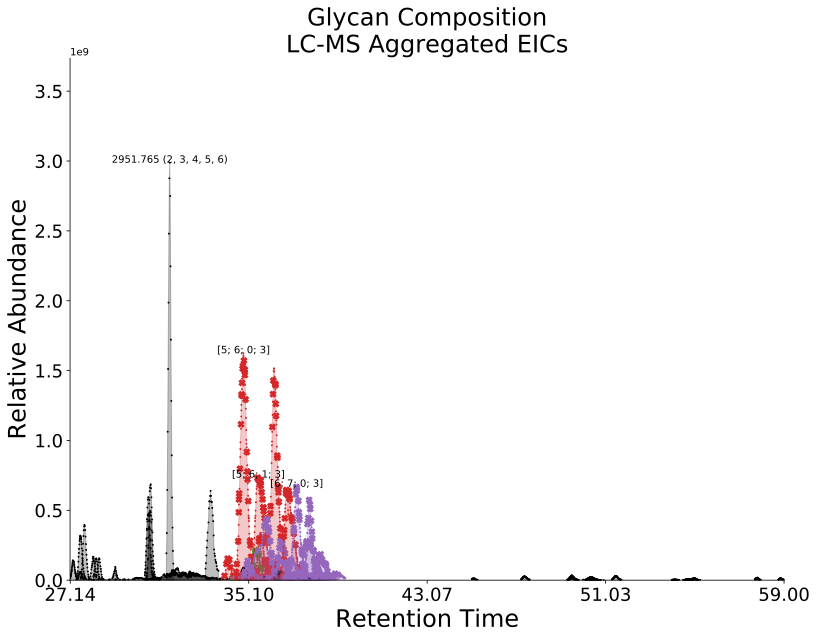
\includegraphics[width=0.45\textwidth,valign=t]{figure/dp_agp_chromatograms.pdf}
        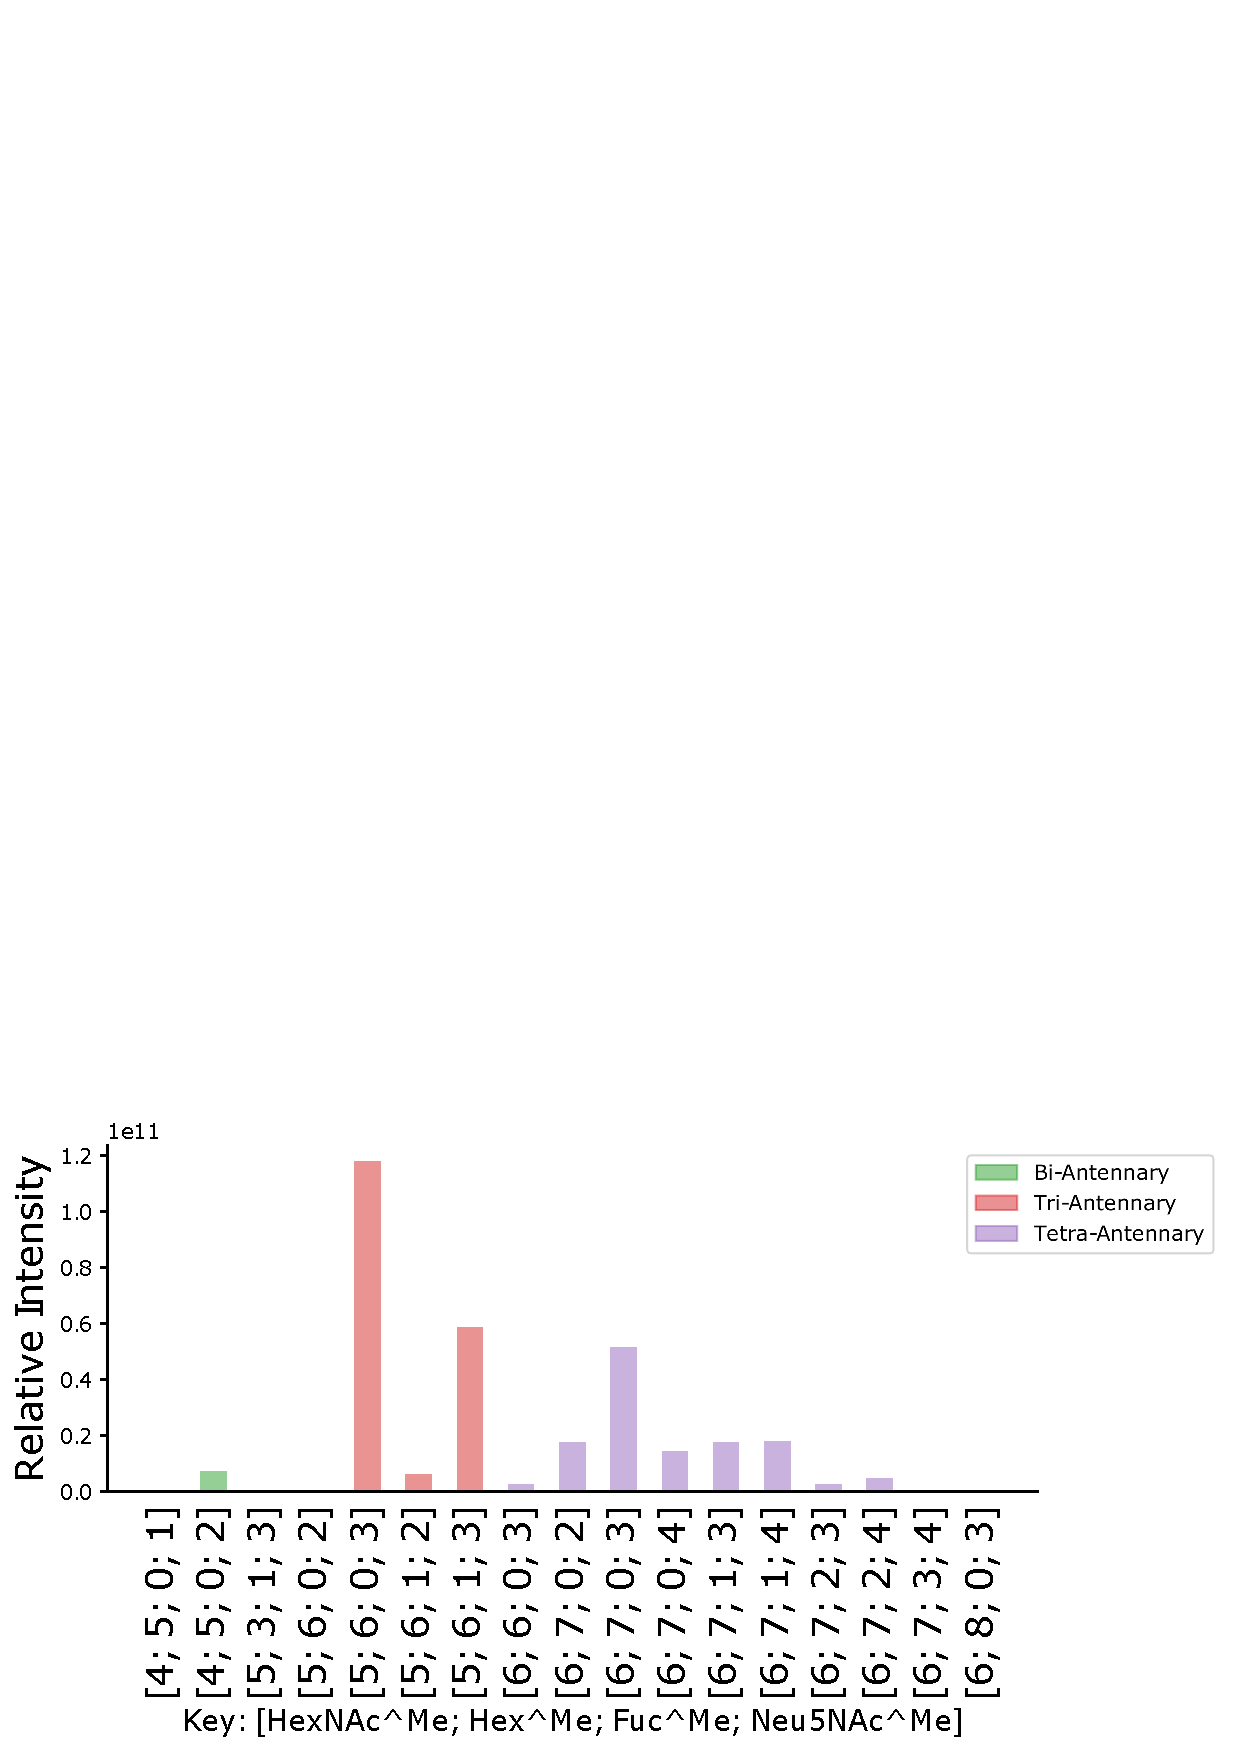
\includegraphics[width=0.45\textwidth,valign=t]{figure/dp_agp_abundances.pdf}
        \caption{\textit{AGP-DR-Perm-glycans-1} Glycan Relative Abundances}
        \label{fig:dp_agp_aggregated_eics}
    \end{figure}

    \begin{table}
        \begin{minipage}[t]{0.25\linewidth}
            \vspace{0pt}
            (a)
            \centering
            
    \begin{tabular}{l | c}
        Group & $\tau$ \\
        \hline
        high-mannose & 0.00 \\
        hybrid & 7.67 \\
        bi-antennary & 15.20 \\
        asialo-bi-antennary & 0.00 \\
        tri-antennary & 22.11 \\
        asialo-tri-antennary & 0.00 \\
        tetra-antennary & 14.57 \\
        asialo-tetra-antennary & 0.00 \\
        penta-antennary & 8.22 \\
        asialo-penta-antennary & 0.00 \\
    \end{tabular}
    
            
        \end{minipage}
        \hspace{1cm}
        \begin{minipage}[t]{0.55\linewidth}
            \vspace{0pt}
            (b)
            \centering
            
    \begin{footnotesize}
    \begin{tabular}{l|p{2cm} p{2cm}}
Glycan Compostion &  Unregularized Score &  Regularized Score \\
\hline
\{Hex:5; HexNAc:4; Neu5NAc:2\}        &                18.73 &              13.71 \\
\{Fuc:1; Hex:5; HexNAc:4; Neu5NAc:2\} &                 4.28 &              11.87 \\
\{Hex:5; HexNAc:5; Neu5NAc:2\}        &                 9.36 &              16.09 \\
\{Fuc:1; Hex:5; HexNAc:5; Neu5NAc:2\} &                 6.60 &              15.61 \\
\{Hex:6; HexNAc:5; Neu5NAc:2\}        &                18.70 &              17.12 \\
\{Hex:6; HexNAc:5; Neu5NAc:3\}        &                20.89 &              17.53 \\
\{Fuc:1; Hex:6; HexNAc:5; Neu5NAc:2\} &                 8.45 &              15.93 \\
\{Fuc:1; Hex:6; HexNAc:5; Neu5NAc:3\} &                19.75 &              17.33 \\
\{Hex:7; HexNAc:5; Neu5NAc:3\}        &                 8.29 &              17.20 \\
\{Hex:7; HexNAc:6; Neu5NAc:1\}        &                 8.48 &               5.81 \\
\{Hex:7; HexNAc:6; Neu5NAc:2\}        &                19.28 &              16.27 \\
\{Hex:7; HexNAc:6; Neu5NAc:3\}        &                19.70 &              16.11 \\
\{Hex:7; HexNAc:6; Neu5NAc:4\}        &                18.42 &              16.03 \\
\{Fuc:1; Hex:7; HexNAc:6; Neu5NAc:2\} &                 9.07 &              15.04 \\
\{Fuc:1; Hex:7; HexNAc:6; Neu5NAc:3\} &                14.38 &              15.45 \\
\{Fuc:1; Hex:7; HexNAc:6; Neu5NAc:4\} &                15.64 &              15.52 \\
\{Fuc:2; Hex:7; HexNAc:6; Neu5NAc:3\} &                10.21 &              15.06 \\
\{Fuc:2; Hex:7; HexNAc:6; Neu5NAc:4\} &                14.24 &              15.12 \\
\{Fuc:3; Hex:7; HexNAc:6; Neu5NAc:4\} &                 7.55 &              14.38 \\
\{Hex:8; HexNAc:7; Neu5NAc:3\}        &                 7.12 &              10.75 \\
\{Hex:8; HexNAc:7; Neu5NAc:4\}        &                 6.38 &              10.56 \\
\{Fuc:1; Hex:8; HexNAc:7; Neu5NAc:4\} &                 5.68 &              10.58 \\
\end{tabular}

    \end{footnotesize}
    
        \end{minipage}
        \caption{
                 Search Results for \textit{AGP-DR-Perm-glycans-1}.
                 (a) Estimated $\mathbf{\tau}$ for grid with ${\hat \gamma} = 16.783889$.
                 (b) Scores For Identified Glycans of grid with ${\hat \lambda} = 0.99$.}
        \label{tbl:dp_agp_score_table}
    \end{table}
